\chapter{Network Compilation}
\section{Layer Decomposition}

\section{Descriptor Generation}
\label{chap:sams:acc_scheduling}

We can generate descriptor programs for the memories (now referred to as SAMs)
in the final architecture template discussed in \autoref{chap:hw_dse:intro}.
These descriptor programs will be used to perform memory operations necessary
for the convolution operation to take place in the final architectural template.
Since we have two operational modes based on the discussion in
\autoref{chap:dataflow_dse:intro} 1x1/GEMM and 3x3 convolutions we will discuss the
descriptor programs required for both of these modes to take place independently of
the other. In both modes we will first highlight the memories participating in
the operation followed by the required descriptor programs for each of those
memories. Please note that muxing plays a part in coordinate the transfer of
data between different memories. The programming of muxes in tandem with SAMs is
left as part of future work. Additionally, all interactions between SAMs and
DRAM are left as part of future work. IFmap and OFmap data is assumed to be read
from and written to DRAM before and after the operation of the SAM programs
discussed in thi section. Latencies and energy penalties associated with DRAM
will be considered in \autoref{chap:hero} but SAM program generation discussed
here is DRAM agnostic.

\subsection{1x1 convolution programs}
\label{chap:sams:acc_scheduling:1x1}

To illustrate how SAMs can be programmed to perform a 1x1 convolution we will
use the final architecture in \autoref{chap:hw_dse:intro} and a 1x1 convolution
layer with 16 channels and 8 filters as a driving example. In
\autoref{chap:hw_dse:intro} there are a total of 9 processing engines with all 9
mapped to the accelerator horizontal spatial axis which enables creates an
effective an unroll factor of 9 at kernel sizes 1x1. Based on the tiling
discussion in
\autoref{chap:dataflow_dse:pruning:applying_it:loop_unroll_factors}, the
architecture tiles the weight tensor into 16 tiles (padding included) as
illustrated in \autoref{fig:1x1conv_sched_tiling}.

\begin{figure}[ht]
    \centering
    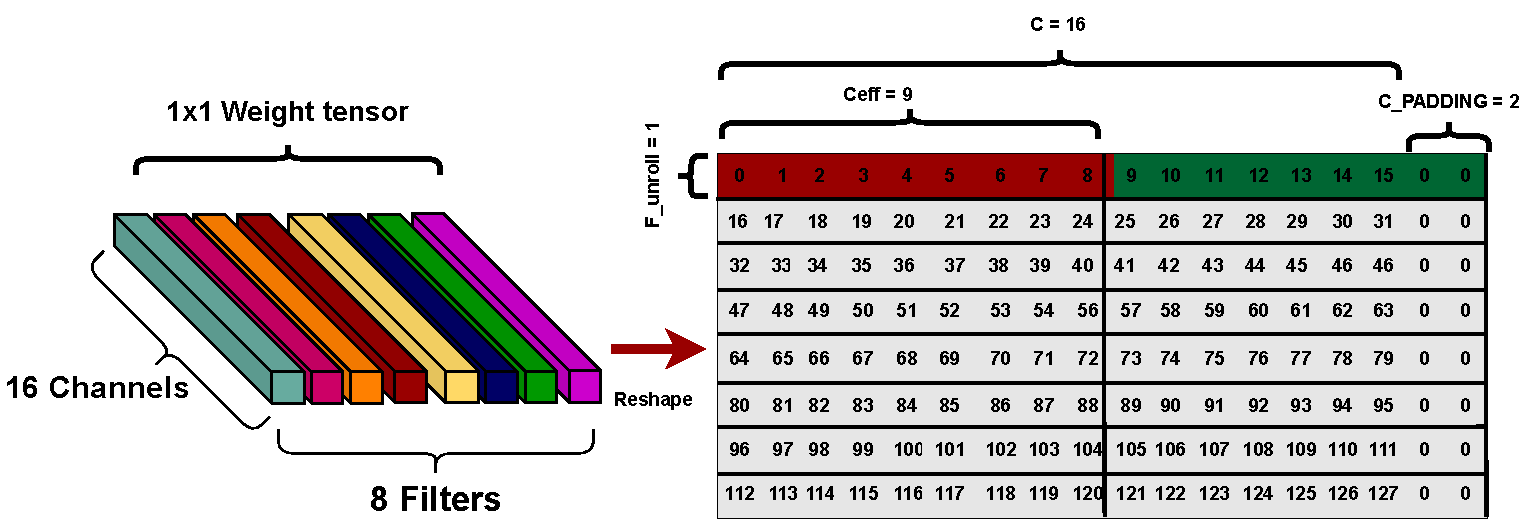
\includegraphics[scale=0.6]{fig/1x1conv_sched_tiling.pdf}
    \caption{Hardware Implementation Taxonomy adapted from \cite{maestro}}
    \label{fig:1x1conv_sched_tiling}
\end{figure}

For each weight in the tiles of \autoref{fig:1x1conv_sched_tiling} the channel
feature map corresponding to that weight has to be streamed into the PE
processing the output of that weight. For example, tile highlighted in red needs
channels C0-C8 streamed into the PEs storing those for processing. After the red
tile is processed, the green tile is loaded into the PEs weight buffer (assuming
ASAP scheduling as seen in
\autoref{chap:dataflow_dse:pruning:applying_it:loop_ordering}). Channels C9-C15
then needs to be streamed into the PEs holding the weights corresponding to
those channels. This means that channel memories may need to hold multiple
channels that are streamed out depending on the index of the tile being
processed. An illustration of how channel feature maps are stored on the channel
SAMs is present in \autoref{fig:channel_banking}. PEs holding 0 valued weights
due to padding have no corresponding channel data so nothing is streamed into
them as reflected in the 0 padding of the last channel SAM attached to the 9th
PE in \autoref{fig:channel_banking}. Additionally, they are assumed to just
forward any partial sums/ output feature maps recieved from their input to their
output with no modifications.

\begin{figure}[ht]
    \centering
    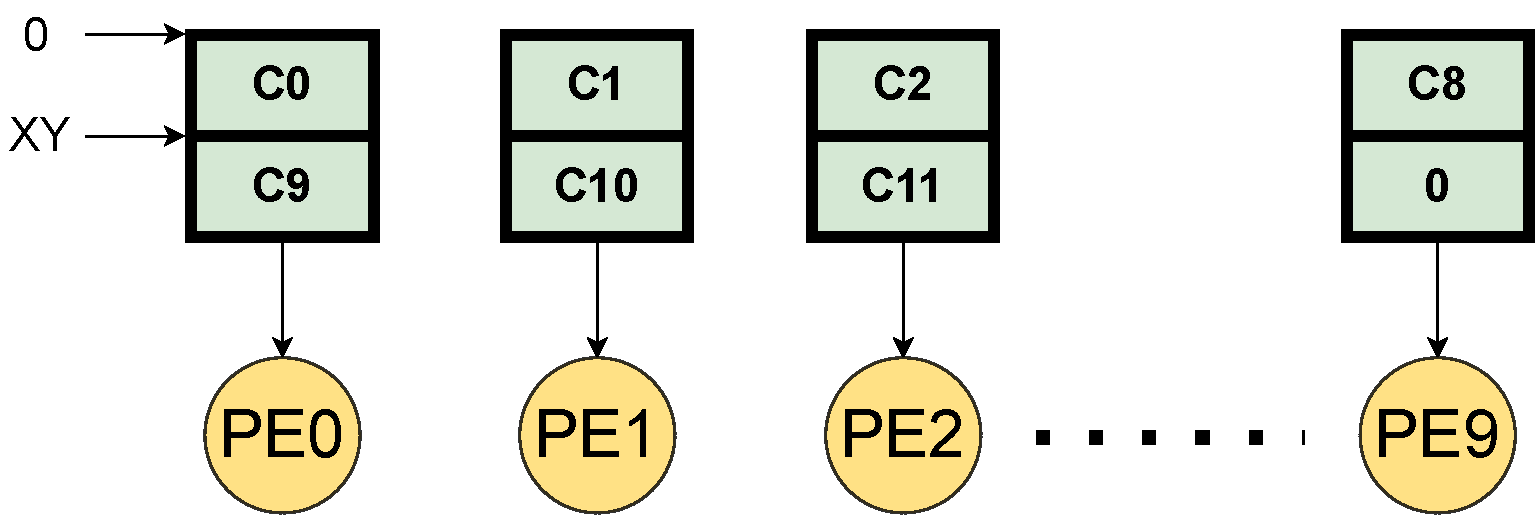
\includegraphics[scale=0.495]{fig/1x1conv_ifmap_banking.pdf}
    \caption{Hardware Implementation Taxonomy adapted from \cite{maestro}}
    \label{fig:channel_banking}
\end{figure}

Since 1x1 convolutions involve entire channel feature maps streamed into PEs
with no reuse within a feature map occuring as in the 3x3 case, the only
memories that need to be programmed are the L3 channel memories and the OFmap
memories. An illustration of the required descriptor programs for the
afformentioned memories is given in \autoref{fig:1x1conv_sched}. In
\autoref{fig:1x1conv_sched} irrelevant layers and muxing as well as some PEs
have been ommited to for brevity.

\begin{figure}[ht]
    \centering
    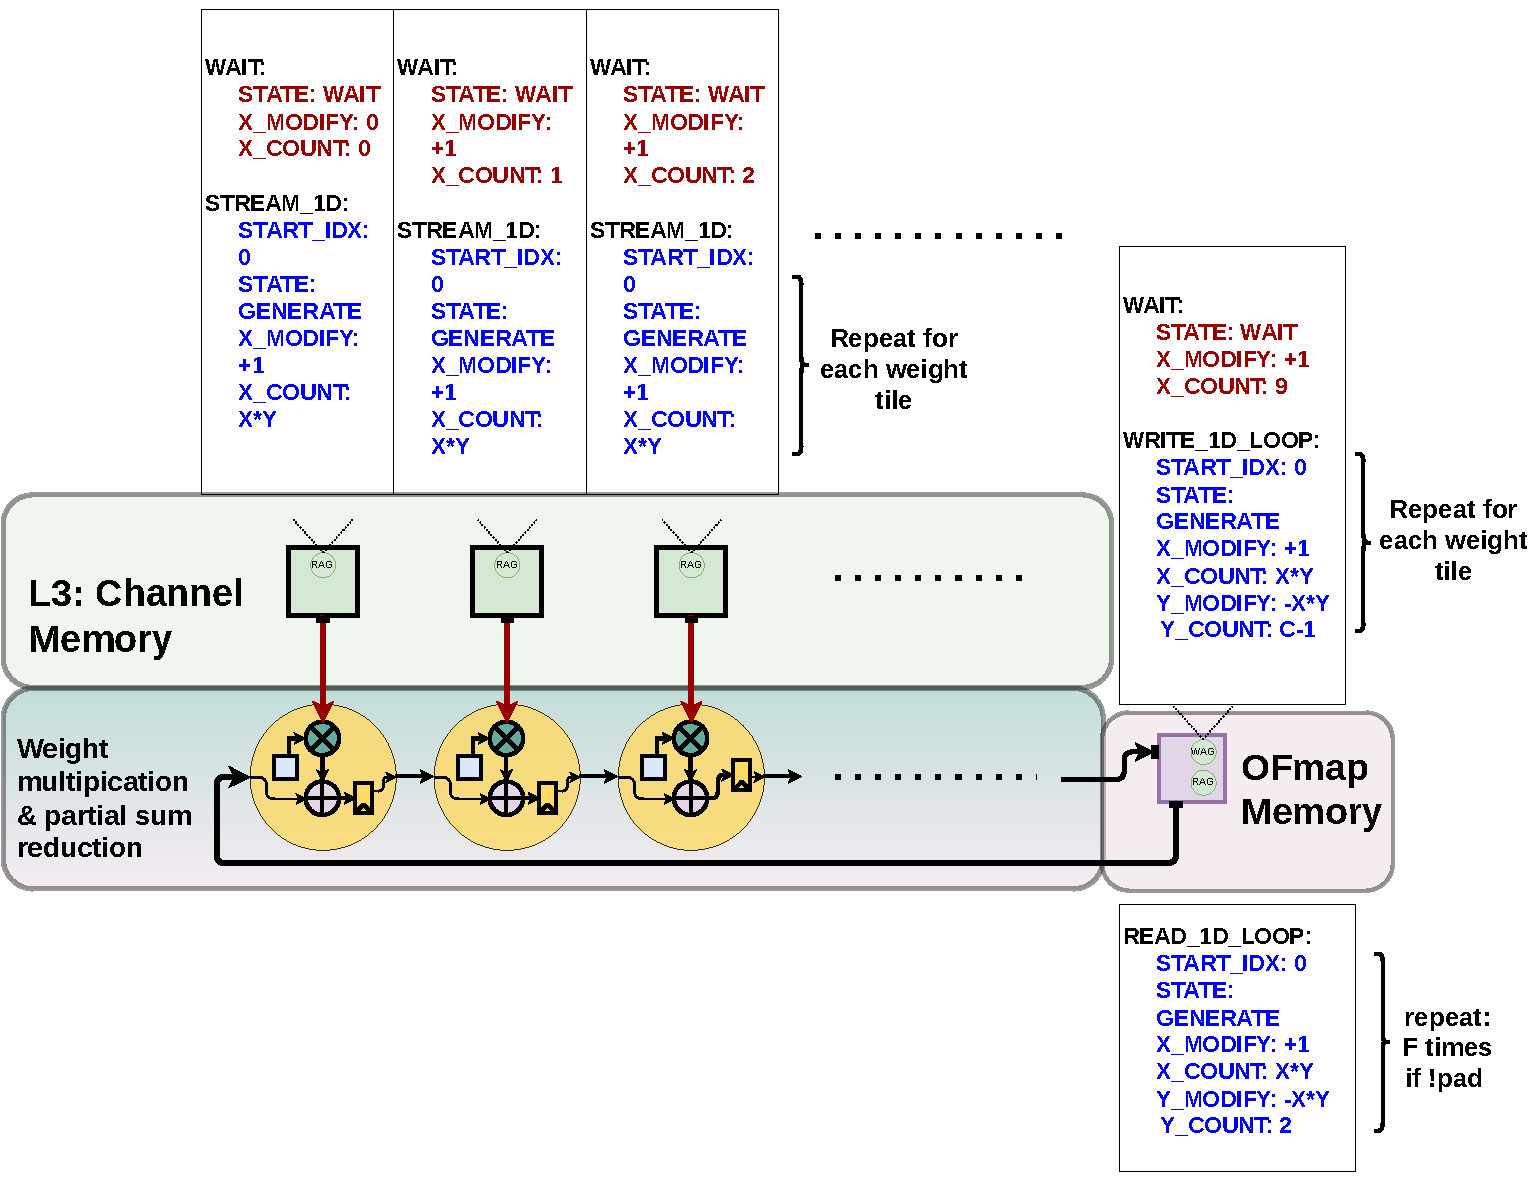
\includegraphics[scale=0.495]{fig/1x1conv_sched.pdf}
    \caption{Hardware Implementation Taxonomy adapted from \cite{maestro}}
    \label{fig:1x1conv_sched}
\end{figure}

In \autoref{fig:1x1conv_sched} channel memories can be implemented with SAMs.
For each channel SAM there are two descriptors types that appear frequently in
their programs, a wait descriptor and generate descriptor. Channel SAMs need to
perform timed reads due to the systolic delays arising from the systolic
reduction of partial sums into output feature maps. Therefore, an initial wait
instruction due to the systolic delay required by each SAM is inserted at the
begining of their descriptor programs. The delay defined by the wait descriptor
for each SAM depends on the index of the PE that the SAM is connected to. So the
first PE's corresponding SAM has no read delay so the x\_count variable in the
wait descriptor is set to 0. The next PE's channel SAM has a delay of 1 so it's
initial weight descriptor's x\_count is set to 1. After the initial wait
descriptor, each channel SAM needs to stream out a feature map. Depending on the
index of the tile being processed, each SAM streams out a different IFmap. What
distinguishes each IFmap stored on a channel SAM from another is it's start
index. For example, for the first tile highlighted in red, the first PE streams
out the IFmap begining at start index 0 with a generate descriptor. The size of
that IFmap is assumed to by $XY$ where $X$ and $Y$ are the width and height of
the IFmap. The generate descriptor increments the internal address "addr" $XY$
times with "addr" starting at 0. The corresponding generate descriptor that
manipulates the "addr" like that is a generate descriptor with an x\_count of
$XY$ and a start index of 0. When the first PE begins processing the second
tile, it reads out the IFmap stored at index $XY$ or more generally
$MOD(tile_{idx},2).XY$ since each filter has 2 tiles. This generate descriptor
is repeated for each tile in the weight tensor assuming that no padding. If a PE
is storing a 0 valued weight due to padding the generate descriptor is replaced
with a wait descriptor with an x\_count of $XY$. Optimizating descriptors to
reduce code size is left as part of future work.

For the OFmap SAM two address generators are required due to the read modify
write nature of OFmaps. The read port begins reading the layer bias immediately
and streams it into the first PE as part of partial sum reduction. All later
reads from the OFmap SAM are for partial sums that have yet to be accumulated
into OFmaps. The read descriptor required for streaming in bias/ partial sums is
a generate descriptor that streams out the contents of OFmap in a loop. It
achieves this by setting x\_count to $XY$ to stream out partial sums of size
$XY$ and y\_count to 2 which the number of tiles in a filter. To reset the
"addr" index of the read descriptor the y\_modify is set to $-XY$. This generate
descriptor is repeated 8 times where 8 is the number of filters present
processed by the PEs assuming no filter padding. Assuming ASAP scheduling as
discussed in \autoref{chap:dataflow_dse:pruning:applying_it:loop_unroll_factors}
OFmaps are written to DRAM as soon as they are completed and are not kept on
chip.

The write port waits for $C_{UNROLL}$ number of cycles to write the first
partial sums that will eventually become OFmaps once the filter being processed
concludes. IFmaps of $XY$ size less than 9 (the number of PEs in the horizontal
axis) will cause additional delay cycles to be introduced via wait descriptors
to allow partial sums to propogate through the PEs to reach the OFmap. The
reduction performed by the PEs are sequential and not combinatorial, hence the
inclusion of registers between each PE. Alleviating dead cycles due to smaller
input feature maps is left as part of future work. The descriptor required for
the write address generator are similair to the the read ones with the exception
of an additional wait descriptor that gives the first partial sum/ Ofmap time to
propogate through the systolic reduction. The delay required by the wait
descriptor is equal to the number of PEs present in the horizontal axis. After
the wait descriptor comes a generate descriptor that writes the partial sum
output/ OFmap output into the OFmap SAM in a loop. The write generatord
descriptor is repeated 8 times as well assuming no padding similair to
the read generate descriptor loop.

\subsection{3x3 convolution programs}
\label{chap:sams:acc_scheduling:3x3}